\section{基于 BIM 的跌落危险检测和\\预防规划案例研究的经验教训}
\subsection{案例研究 1:手工建模与自动建模的比较}

在第一个案例研究中,对办公楼地下室现浇混凝土的防坠落设备进
行了人工和自动建模。比较了两种方法的优缺点。\\

(1)安全防护装备的手工模型:\\

为了了解安全预防系统建模和计划编制工作的复杂性,图 \ref{fig:c4f1} 首先在 BIM
中进行了人工建模和计划编制。展示了一张照片和模型化的 3D 安全栏
杆组件,因为它通常用于芬兰的建筑项目。所选择的护栏解决方案为领
先的边缘板表面包括护栏的职位和木材栏杆。定制安全部件的 3D 表示
是手工建模的。现实的护栏解决方案是基于最佳实践信息承包商提供并
在建筑工地使用。职位的几何对应的芬兰 Vepe 产品。扶手、中间护栏
和脚趾板的尺寸与现有规格相符。

\begin{figure}[thbp!]
    \centering
    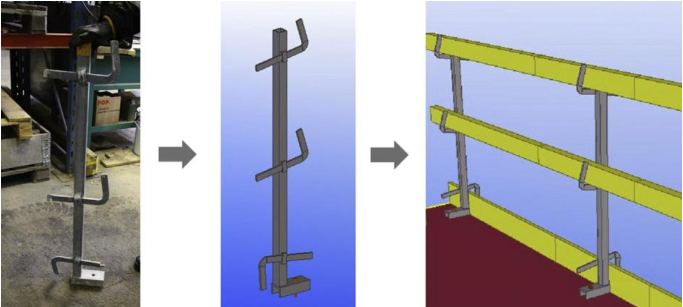
\includegraphics[width=1.0\linewidth]{res/c4f1.png}
    \caption{工程安全护栏设备模型(表面安装护栏柱与木质护栏一起使用)}
    \label{fig:c4f1}
\end{figure}

其想法是在板边缘规划护栏柱的位置,以便在施工期间无需移动护栏柱。
这样既可节省时间,又可减低从高处堕下的风险。如果
栏杆靠近混凝土柱(见图 \ref{fig:c4f2}),栏杆柱与设计柱之间有一定距离。
在钢梁上有预制孔的前缘使用相同的安全栏杆解决方案,确保安全设备的快速安装和拆卸(见图 \ref{fig:c4f3})

\begin{figure}[thbp!]
    \centering
    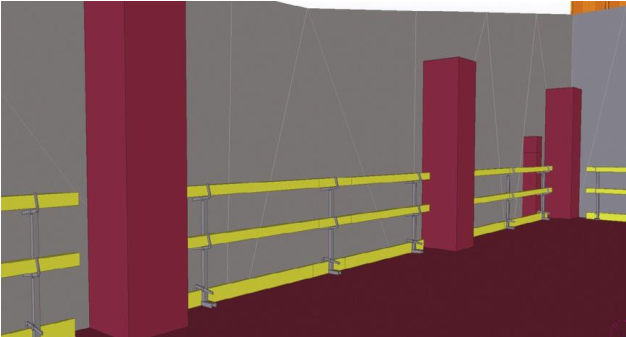
\includegraphics[width=1.0\linewidth]{res/c4f2.png}
    \caption{基于 BIM 的防坠计划:现浇板边缘的安全栏杆)}
    \label{fig:c4f2}
\end{figure}

\begin{figure}[thbp!]
    \centering
    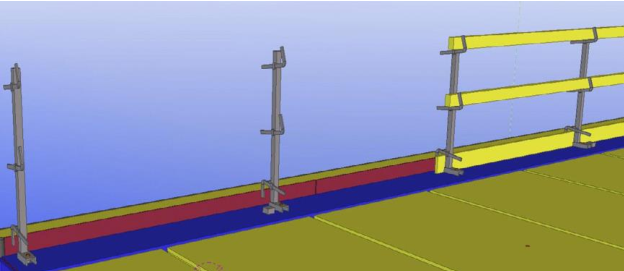
\includegraphics[width=1.0\linewidth]{res/c4f3.png}
    \caption{同样的安全栏杆解决方案模拟到上层办公楼:护栏柱安装在预制钢梁的预先设计孔中)}
    \label{fig:c4f3}
\end{figure}

手动生成的基于 BIM 的安全护栏平面图连同一些模型视图一起交付给承包商,
这些模型视图提供了在现场实施的模型化解决方案。
由于临时安全设备的 4D 调度与当前的BIM建模工具复杂,
VTT 研究团队将混凝土和钢框架施工相关的防坠落可视化,
并将永久性建筑结构和任何临时安全设备的工作流程计划和可视化。

在实际试验开始之前,对项目中的 4D BIM 工具的使用进行了功能测试。
测试项目是一个办公楼,最初是由该项目的结构工程师使用 Tekla Structures 软件建模。
结果表明,交互式4D坠落防护规划,特别是安全栏杆的调度和可视化,为实际工作者提供了一种可行的方法。

从实际出发,为了实现基于4D BIM的临时结构规划和可视化,
需要对其建模和可视化进行一些特殊的要求或设置。
例如,在4D模拟方面,临时结构在不再需要后需要从模型中移除或者是隐藏。\\

(2)基于规则检测算法的跌落危险自动检测与防护\\

人工建模的坠落防护方法提供了对施工现场潜在坠落危险的良好理解,通常具有较高的详细程度。
但是,由于手动建模的耗时性,建议使用自动建模方法。本文提出的系统已在同一试点工程中得到应用。
图 \ref{fig:c4f4} 展示了开发的系统在地下室一层的自动建模结果。\\

\begin{figure}[thbp!]
    \centering
    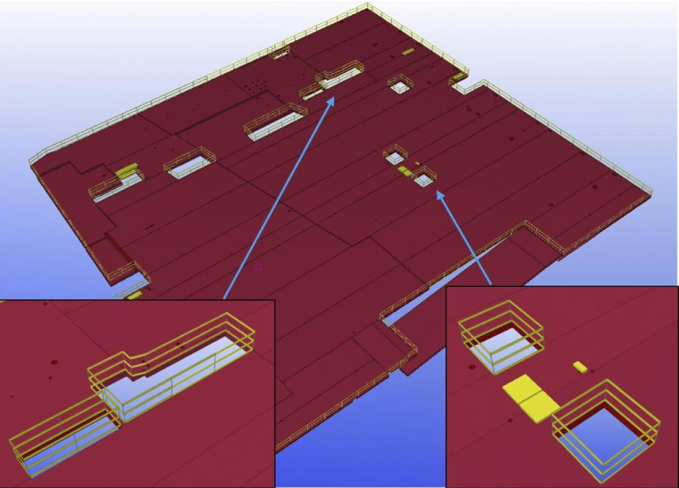
\includegraphics[width=1.0\linewidth]{res/c4f4.png}
    \caption{板边孔自动检测及护栏安装效果}
    \label{fig:c4f4}
\end{figure}


(3)基于手动 BIM 跌落保护方法建模经验\\

通过建立同一办公楼结构模型中的安全栏杆和楼盖模型,进行了跌
落危险的检测和防范规划。这种规划比传统的人工规划更为详细。

现场工作人员指导研究组实施的规划和建模。该规划和建模工作比工作阶段的开始早了三个月。
在目前的规划实践中,此类详细的防坠落规划并没有在项目阶段的早期进行。
只选择和采购所需的安全设备类型,并提出了更全面的防坠落安排计划。

图 \ref{fig:c4f5} (a-j) 展示了如何在 BIM 和施工现场实施基于模型的防坠落计划。
由于视角稍有不同,图片之间存在一些视觉差异。一些图片还展示了混凝土模板的模型。
当它影响到安全栏杆的位置时,它的各个部分的建模要比安全栏杆更抽象。

\begin{figure}[thbp!]
    \centering
    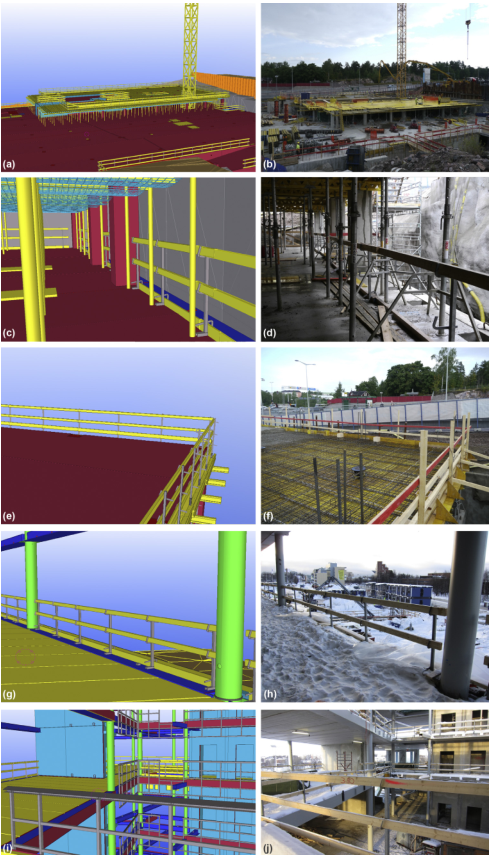
\includegraphics[width=0.8\linewidth]{res/c4f5.png}
    \caption{比较模型和现场情况:a,b 为地下室施工阶段试验现场的一般视图;c,d 是板前缘;e,f为混凝土板模板;g,h是安全轨柱用螺栓连接到钢梁上的焊接螺纹套筒,以及 i,j 为办公楼的中庭临时防坠落系统的一般视图)}
    \label{fig:c4f5}
\end{figure}

目前的一个区别是,材料、设备和其他暂时性的构造对象并没有在 BIM 中建模。
然而,由于这些对象可能是事件的参与者或导致事件发生,因此也应该对它们进行建模。
分析行业的详细工作活动和空间需求可能是有用的,因为行业在本质上是高度动态的。
这些问题都不在本文的讨论范围之内。

板边缘安全栏杆的位置与平面图相比发生了实质性的变化(见 图 \ref{fig:c4f5} c 和 d)。
计划位置的最初想法是允许在靠近边缘的栏杆后面安装墙构件。
在现场安全栏杆的实施阶段,决策者决定将护栏进一步放置在板内,以便栏杆形成连续的护栏。

临时楼梯是地下室较低楼层的紧急出口,如图 \ref{fig:c4f6} 所示。
由于脚手架建模需要其他工具,因此在建模时未计划设置护栏。改变安全栏杆位置的一个主要原因是占地面积需要三条腿支撑架的空间。
一旦护栏向内移动,中间的栏杆必须拆除。另一个原因可能是,
规划期间使用的最新 BIM 版本的结构模型确实包含了几个用于将立面元素固定到楼板边缘的方孔。

\begin{figure}[thbp!]
    \centering
    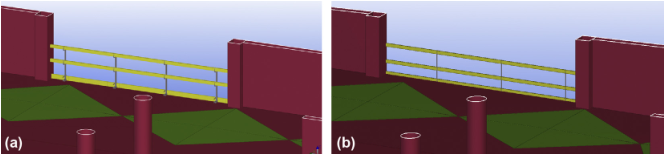
\includegraphics[width=1.0\linewidth]{res/c4f6.png}
    \caption{(a) 手动与(b)自动建模结果}
    \label{fig:c4f6}
\end{figure}

这些孔限制了护栏安装的可用区域。此外,由于安全规划是在施工前三个月完成的,
因此最近的变更可能不会在 BIM 中实施。因此,使用 BIM 的详细安全隐患检测和预防计划应始终接近施工,
并使用最新和最新版本的 BIM。基于 BIM 的详细安全规划还应与所有项目干系人,
特别是最终负责安全设备实施的分包商进行协调。其他风险可能与使用其他工具类似。
管理人员应当把建模结果作为最终确认的结果,当建模结果提示为危险时应该完全信任他;
现场应该使用软件测算的结果来管理,应该避免管理者使用他们自己的的技能和经验。

在许多项目中,设计方案和施工方案也可能不同。混凝土板前缘的安全栏杆(见\ref{fig:c4f5} e 和 f)在设计方案上是金属柱和木制护栏。
然而,在现场施工则使用了一种使用木桩作为临时的解决方案。
如果不遵守标准,偏差就可能会导致严重的安全问题。这种偏差和材料更换需要现场人员解释情况。
在现场使用人造安全设备当然不遵循安全规定,除非是为了克服不可预见的现场条
件。
图 \ref{fig:c4f5} 的 g 和 h 显示了试点项目的一个上层的安全栏杆,它使用了一种栏杆的解决方案——
即用螺栓将立柱连接到钢梁的螺纹套筒上。这些固定件焊接到钢制车间的钢梁上。
它们已经出现在钢框架的结构模型中,套筒为栏杆柱提供了一种快速可靠的固定方法。
选定的工艺有利于安全安装和拆除安全栏杆,特别是在恶劣的现场条件(即天气)下。


试点大楼的内部有一个中庭空间,每一层都需要防坠落装置。设计
的 BIM 模型建议在钢结构安装完毕后立即安装最终的护栏系统。这可以
通过在吊装到位之前将护栏预先焊接到钢材上来实现。
然而,最初设计
的解决方案并没有在年实施由于护栏类型的改变而造成的场地。承建商不得不对这一变化迅速做出
反应,并在施工期间实施了传统的护栏系统,后来被永久护栏系统所取
代(见图 \ref{fig:c4f5} i 和 j)。设置临时护栏系统的另一个常见原因是为了避免在施工过
程中损坏固定的永久护栏。在这两种情况下,规则检查系统都可以有效
地生成解决方案。\\

(1) 人工与自动落地保护模型建立方法的比较\\

自动建模方法的优点如下(见表\ref{tb:compare}):(1)使用自动建模方法所需的时间比手
动建模大大减少。对于像案例研究项目这样复杂的建筑模型,通常需要
几秒或几分钟才能生成结果。
手动建模需要更高的安全专业知识和建模熟悉程度。建模人员需要充分
理解模型,知道如何添加和调度栏杆组件,更重要的是,建模人员需要
熟悉安全规则和需求。然而,安全专门知识并不是自动化方法的必要先
决条件,因为已知边界已经存储在系统中并编入程序。(3)一旦进行了设
计变更或进度更新,手工更新相应的安全要求是困难和耗时的。相反,
自动安全检查系统可以很容易地重新启动以生成新的结果。(4)手动建模
可以提供更高层次的细节的安全解决方案(见)。在施工柱和墙体之前,
板边护栏需要拆除。在(a)项中,栏杆柱被小心地安置在靠近柱子的位置,
这样以后就不需要额外的柱子了。然而,自动化建模并没有考虑这些细
节。在(b)中,在柱和墙的结构完成后,需要在靠近左侧柱的地方增加一
个柱子。针对护栏无法延伸一定距离,必须自动设立立柱的问题,提出
了一种解决方法。

\begin{table}[thbp]
    \caption{手工和自动建模方法的比较}
    \begin{center}
        \begin{tabular}{@{}lcc@{}}
            \toprule
            \multicolumn{1}{c}{\textbf{}} & \textbf{手工建模} & \textbf{自动建模} \\ \midrule
            \textbf{时间需求} & 长 & 短 \\
            \textbf{安全知识需求} & 非常多 & 少 \\
            \textbf{更新困难性} & 困难 & 简单 \\
            \textbf{细节的等级} & 高 & 低 \\ \bottomrule
            \end{tabular}
    \end{center}
    \label{tb:compare}
    \end{table}

\subsection{案例研究 2:BIM 中的动态跌落危险检测和预防}

在第二个案例研究中,开发的自动规则检查工具应用于多层预制公寓建筑模型(见图 \ref{fig:c4f7})。
目标是根据项目进度动态演示安全检查结果。所有预制混凝土构件均已制造并运至施工现场,
并将按照预先确定的顺序从 A 部分开始安装,然后是 B 部分和 C 部分。预制混凝土就位后,
在现场建造外墙保温层和砖墙。该项目的结构模型已使用 Tekla Structures 17.0 建模软件进行建模。
开发的自动规则检查平台所需的4D进度表是根据从承包商获得的信息添加到结构模型中的。
该信息由现场工程师以施工进度表和涉及安装顺序的工作分解结构(WBS)的传统格式提供。

\begin{figure}[thbp!]
    \centering
    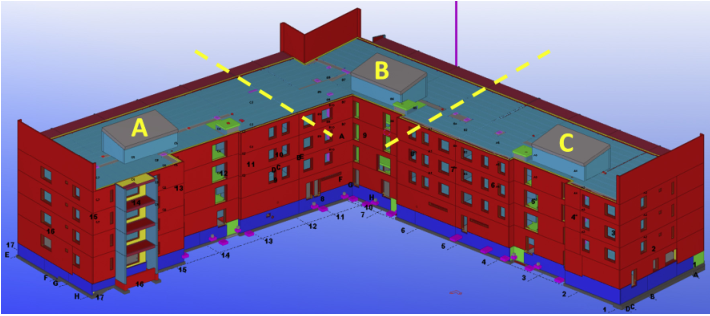
\includegraphics[width=1\linewidth]{res/c4f7.png}
    \caption{多层预制公寓建筑模型及其剖面图}
    \label{fig:c4f7}
\end{figure}


图 \ref{fig:c4f8} 可以近距离观察到混凝土板块。在楼板安装完毕之后,对楼板的连
接部分进行加固和浇筑,而在下一层楼板安装之前,墙板安装已经开始。
墙体和升降机井与楼板一起作为一个结构系统工作,将荷载传递到基础
上。楼板部分是按层安装的。一个截面的一层楼大约需要7天的时间,
一个截面的搭建大约需要 5-6 周的时间。护栏解决方案需要根据板截面的增长进行更新,
例如,当两个板截面在同一水平面上合并时,需要移除中间的护栏。

\begin{figure}[thbp!]
    \centering
    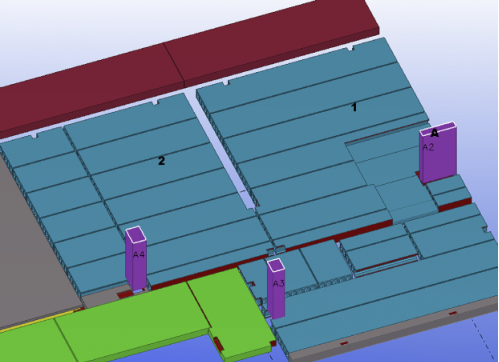
\includegraphics[width=0.8\linewidth]{res/c4f8.png}
    \caption{预制板面板近景}
    \label{fig:c4f8}
\end{figure}
\newpage
在完成规则检查算法的基础上,它实现了包括护栏在内的防坠落系统
的自动可视化。

它还为在施工进度中安装和拆除安全相关设备创建了子任务。并
将其纳入施工进度表。
图 \ref{fig:c4f9} 示出了部分更新的具有所需安全解决方案的时间表。
图 \ref{fig:c4f10}示出了模型模拟的四个不同阶段,
可以实现安全设备嵌入模型和施工进度的时间可视化。
4D模拟的对象表示如图 \ref{fig:c4f11} 所示。一楼的楼板从 A 段到 B 段,
由于施工过程中有时会合流,中间的护栏必须拆除,
拆除也改善了现场的工作流程,因为工人现在可以安全地从A段走到B段而不必绕道。
建筑顺序的安装和拆除如图 \ref{fig:c4f12}(a)和(b)所示。

\begin{figure}[thbp!]
    \centering
    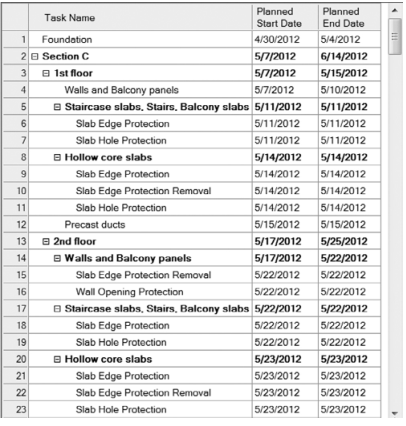
\includegraphics[width=0.8\linewidth]{res/c4f9.png}
    \caption{更新的包括防坠落方法的安装和拆除的施工进度表}
    \label{fig:c4f9}
\end{figure}

\begin{figure}[thbp!]
    \centering
    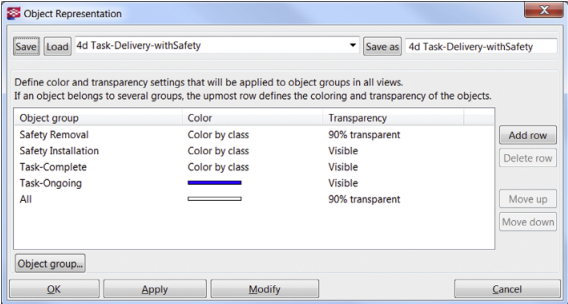
\includegraphics[width=0.8\linewidth]{res/c4f10.png}
    \caption{4D 模拟的对象表示设置}
    \label{fig:c4f10}
\end{figure}

\begin{figure}[thbp!]
    \centering
    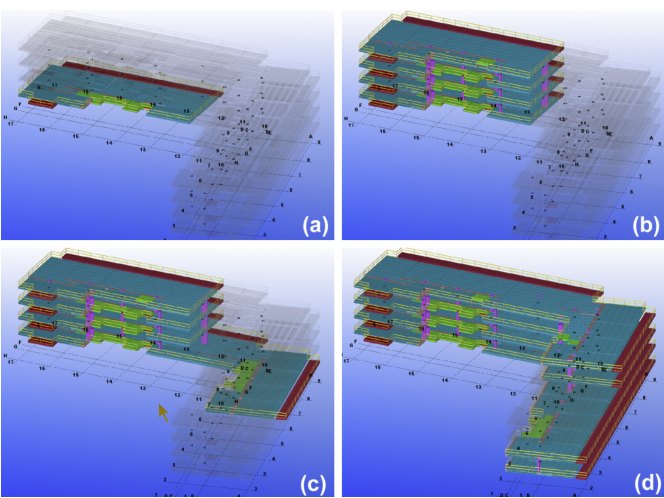
\includegraphics[width=0.8\linewidth]{res/c4f11.png}
    \caption{模型板、柱和护栏防护系统的4D仿真}
    \label{fig:c4f11}
\end{figure}
\newpage
\begin{figure}[thbp!]
    \centering
    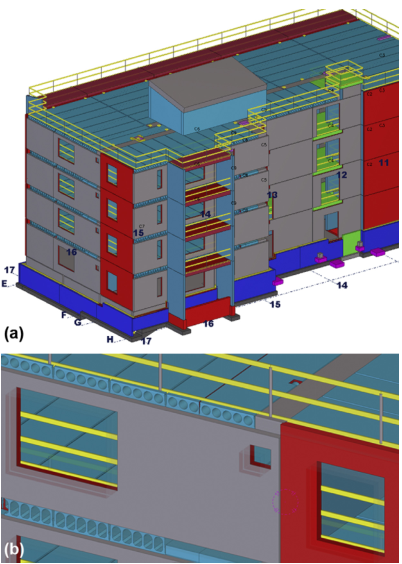
\includegraphics[width=1\linewidth]{res/c4f12.png}
    \caption{(a) 建筑物 a 区的防坠落保护系统和(b)墙洞保护的近景}
    \label{fig:c4f12}
\end{figure}

图 \ref{fig:c4f12} 示出了板边缘保护和墙洞口保护的更详细视图。在模型中生成安全防护系统后,
也会自动生成检查报告。然后,可以将该报告导出为 MS-Excel 格式,如 图 \ref{fig:c4f13} 所示。
这种文件格式允许现场安全或监督人员简化生成数据的使用。
例如,他们可以计算保护工作场所所需的安全设备。
最终,该清单还可能支持详细安全解决方案的预制,这些解决方案可以在场外预制,
并以与定制预制混凝土板类似的方式安装。
因此,开发的工具及其生成的数据支持多种安全设计 (Design-for-Safety,DfS) 概念。
该清单也可用作检查清单,以确保所有必需的安全防护系统已在施工现场到位。

板坯开孔检查的用户界面如图 \ref{fig:c4f14} 所示。用户可以使用工具的界面根据不同的预防方法定义自己的需求。
规则执行后,安全防护设备将在模型中可视化,检查结果将在单独的对话框中列出,
安全管理人员可以从中预览结果,并在必要时手动进行更改。
这使得人类决策者随时处于安全防护危险检测和预防的循环中。

\begin{figure}[thbp!]
    \centering
    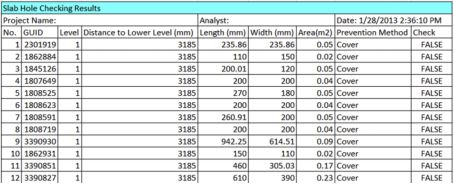
\includegraphics[width=1\linewidth]{res/c4f13.png}
    \caption{材料清单:板孔检查结果为安全设备的估算和预制提供了Excel表}
    \label{fig:c4f13}
\end{figure}

\begin{figure}[thbp!]
    \centering
    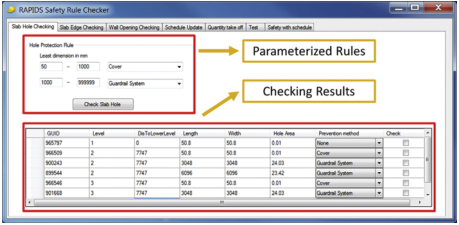
\includegraphics[width=1\linewidth]{res/c4f14.png}
    \caption{板孔检查的用户界面}
    \label{fig:c4f14}
\end{figure}

\newpage
\subsection{讨论}

该工具能够自动、成功地检测出无防护板边缘并安装护栏系统。利
用 BIM 软件的内置功能,可以方便地计算护栏的起吊量。此外,自动安
装的板边缘和窗口护栏可以由用户手动修改。

在试验过程中,工具中成功地集成了所谓钩柱的详细三维模型(见图17)。
用户现在可以为安全扶手建模选择简化的模型表示或详细的表示(自定义构件)。
此外,更详细的护栏模型和相关的安全设备零部件,如焊接配件,
可以自动添加到钢梁或混凝土面板中进行护栏安装建模。
在钢梁或混凝土面板的制作中可以预先考虑相应的连接,从而减少高空作业。
然而,如果用户的目标是提供详细和自动化的安全建模,
那么还需要进一步开发一个程序来改进岗位规则。

目前开发的系统的一个限制是它严重依赖于 BIM 提供的信息,如几何结构和时间表。
如果BIM中的信息不完整、不正确或不准确,安全分析的正确性将受到很大影响。
此外,建筑模型几何结构(例如,具有复杂空间相关性的对象形状)或场地条件
(例如,有助于施工过程且通常未建模的临时结构)可能导致当前版本的规则检查系统的应用失败,
或者最多产生经验丰富的安全专家能够理解和解决的结果。为了获得更准确的结果,
建议首先运行自动系统来对照模型进行检查


目前开发的系统的一个局限性是,它严重依赖 BIM 提供的信息,如
几何图形和时间表。如果 BIM 中的信息不完整、不正确或不准确,安全
分析的正确性将受到很大影响。此外,构建模型的几何形状(例如,具有
复杂空间依赖性的对象形状)或场地条件(例如,有助于构建过程且通常
未建模的节奏元结构)可能会导致规则检查系统当前版本的应用失败,或
者产生经验丰富的安全专家能够理解和解决的最好结果。为了获得准确
的结果,建议先运行自动化系统对照模型进行检查。
安全专家随后会审核结果,并提供意见。目前,Zhang 等人使用开发的原型工具会
自动创建概念性防坠落计划。未来研究的另一个领域是生成工艺流程图,以及安全工程师、专家和检查员的作用,
因为他们应该充分利用基于BIM的安全隐患探测预防规划工具。朝着这一方向迈出的第一步是自动化
工作危害分析(JHA)。\\

根据已进行的测试结果,今后可能需要改进的地方包括:

\begin{enumerate}
    \item 为安全元素提供高层次的细节:例如,例如,护栏的柱子和板子可以通过带
    有抽象线条的 BIM 可视化。
    经验不足的用户可能更喜欢高层次的视觉细节以及它看起来像什么,比如如果需要锚定,
    这些位置需要被确定。有经验的用户可能对附加功能的高层次细节感兴趣,
    例如,当某些安全设备可以预制时。了解护栏柱与建筑构件之间的复杂连接可以加快此类构件在现场的安装过程。
    \item 使用独立于软件的数据交换格式:独立于软件的数据交换格式便于多个项目涉众之间的通信。
    出于安全规划的目的,需要探索一种基于IFC 的解决方案。
    使用 IFC 模型进行自动安全检查和规划的能力将使在
    各种 BIM 模型创作工具中创建的模型具有更广泛的检查能力。
    \item 在复杂模型测试:未来,更全面的基于BIM的防坠落规划解决方案需要在复杂模型几何结构上进行测试,
    并提供全系列安全解决方案的高水平细节。例如,在施工期间以及设施运行和维护期间,
    安装备用解决方案,如安全网和挂钩。
\end{enumerate}